\documentclass[a4paper]{rapport}

\graphicspath{{Pictures/}}

\begin{document}
\part{Quelques notion d'astrophysique}
On appel \textit{Cycle de la matière galactique} les différentes étapes et états par lesquels transite la matière telle que nous la connaissons. C'est par ce cycle que notre univers s’enrichit en éléments lourd et que les étoiles ainsi que tous les objets visible sont créé, il va être question dans cette première partie de décrire ces différentes étapes et de mieux comprendre comment évolue la matière au sein de notre univers.
\nl
Nous allons prendre comme point de départ de notre cycle le \textbf{milieu interstellaire}, il à une masse d'environ $5.10^{9}M_{\odot}$ et est constitué aux trois quart d'hydrogène, d'hélium à niveau d'un quart et que poussière pour ce qui est des dixième de pourcent restant (il constitue le réservoir de matière de notre univers). On considère que dans ce milieu la densité est environ d'une particule par $cm^3$, bien que cela soit extrêmement faible, certaines régions sont plus densément peuplée que d'autres (augmentant la gravité de certaines zones de l'espace) et si l'ont rajoute à cela la dynamique des fluides on observe sur des périodes de temps assez faibles (quelques millions d'année) l'apparition de nuage moléculaire.\\ Ces nuages forment le milieu interstellaire \textbf{dense}, sa masse reste de l'ordre de $10^{9}M_{odot}$ mais sa composition à évolué pour être constitué à environ $75\%$ de dihydrogène (d’où le nom de nuage moléculaire). C'est à partir de ce moment que les choses vont s'emballer, les zones les plus denses des nuages vont attirer plus de matière à eux entraînant une augmentation de la densité etc... jusqu’à ce que l'instabilité gravitationnelle soit trop forte et que le nuage s’effondre sur lui même.\\
Il résulte de cet effondrement, la formation d'une' \textbf{Proto-étoile}. Durant cette phase qui va durer quelques centaines de milliers d'années, la matière va continuer à tourner s'agglomérer autour du centre de gravité. Au fur et à mesurer de ce processus la proto-étoile va voir sa température augmenter, les particules du gaz vont s'échauffer continuellement jusqu’à atteindre une température critique qui permettra "l'allumage" de la réaction de fusion de l'hydrogène, une \textbf{Étoile} est née.\\
Le cycle de vie d'une étoile est assez complexe, pour simplifier nous dirons que l'étoile fusionne de l’hydrogène en son sein et que cette réaction et à l'origine de la pression interne de l'étoile, pression qui vient compenser la force de graviter qui tend à faire s’effondrer l'étoile sur elle-même. Le cycle de vie d'une étoile est représenté par un diagramme HR (\textit{Hertzsprung-Russel}) qui permet de voir l'évolution d'une étoile le long de la séquence principale (où elle passera le plus clair de son existence) mais également de savoir quel objet astronomique il résultera de sa mort.
\begin{figure}
    \center
    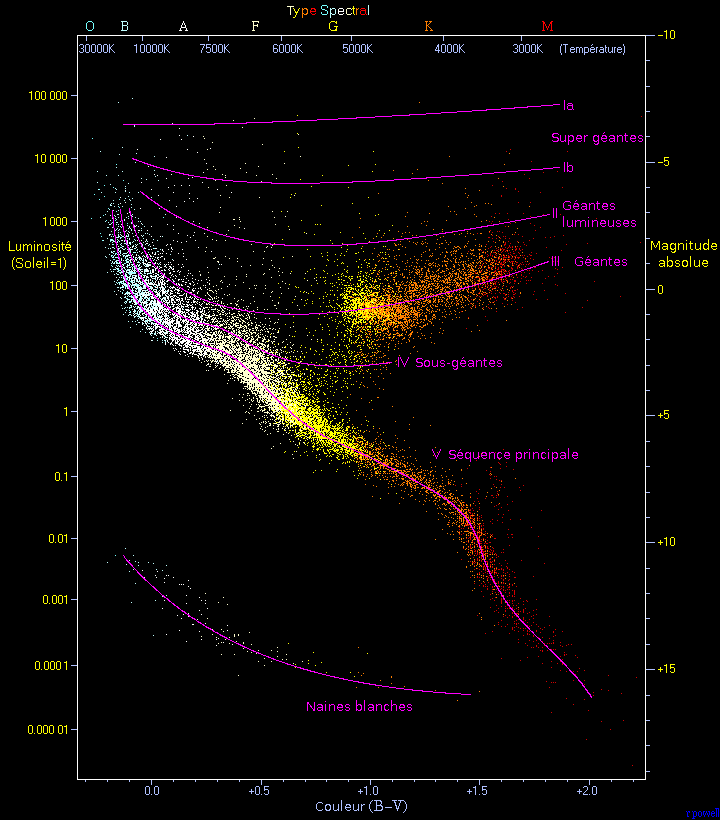
\includegraphics[scale=0.2]{hr_diagram_wikipedia}
    \caption{Diagramme HR représentant la position d'une étoile en fonction de sa magnitude (de haut en bas, des étoiles les plus lumineuse aux moins lumineuses) et de leur couleurs (et donc de leurs températures, les étoiles bleus étant plus chaudes que les étoiles rouges). Source : \url{https://fr.wikipedia.org/wiki/Diagramme_de_Hertzsprung-Russell}}
\end{figure}
Une fois que l'étoile à épuiser tout son hydrogène, la gravité va reprendre le dessus faire s’effondrer l'étoile, augmenter la pression et la température, réunissant les condition pour fusionner l'hélium, stoppant effondrement etc...\footnote{Ce processus s’arrête au fer car aucune étoile ne peut fusionner le fer, en effet la fusion post fer consomme de l'énergie la ou la fusion pré fer en produisait.}. Une fois que l'étoile aura épuisé tout son carburant elle "mourra" sois en passant par la \textbf{Nébuleuse planétaire} sois en \textbf{Supernovæ} si l'étoile était suffisamment massive.\\
Ces deux phénomènes permettent de rendre au milieu interstellaire un grand nombre de nouvelle particules, enrichissant de manière considérable celui-ci et permettant l'apparition future d'objet céleste plus complexe en terme de composition.
\nl
Nous rentrerons plus en détails sur les phénomènes de Nébuleuse planétaire et de Supernovæ dans les parties consacrées aux \textbf{Étoiles à neutron} et au \textbf{Naines blanches}, car nous verrons que dans la plupart des cas \footnote{La réalité astrophysique est bien plus complexe que cela et la manière de former certains objet de notre univers peut être assez exotique.} Ces objets sont le résultats des Nébuleuses et des Supernovæ.

\part{Les naines blanches}
\section{Nébuleuse planétaire}
Comme dit précédemment nous allons revenir sur le phénomène de Nébuleuse planétaire qui donne naissance à la plupart des naines blanches de l'Univers.\nl
Pour commencer il faut savoir qu'une manière de classer les étoiles consiste à les ordonnée selon leurs masse, et donc on estime que seuls les étoiles de masse moyenne (C.à.D de moins de $10M_{\odot}$) donnent naissance à des Naines blanches. Le processus qui mène à la création d'une telle étoile est le suivant.\nl
Tout d'abord comme nous l'avons vu dans notre introduction, une étoile va fusionner son hydrogène en hélium \footnote{On a généralement deux moyen d'y parvenir, sois par cycle proton-proton qui va par le biais du deutérium et du tritium/hélium 3 va donner de l'hélium 4, sois par le cycle CN0}\\
A partir de ce moment, la gravitation redevient alors la force dominante et l'étoile s’effondre sur elle même, les nouvelles conditions de pression et de température permette la fusion de l’hélium \footnote{Par un procédé appelé réaction triple alpha lorsque que la température aura atteint les $10^8 K$} cette fusion produit principalement du carbone et dégage une une importante quantité d'énergie qui ne se contente plus de contrebalancer l'effondrement gravitationnel mais qui fais gonfler l'étoile de manière impressionnante \footnote{On considère que lorsque le soleil entrera dans sa phase de géante rouge, sa taille aura tellement augmenter qu'il atteindra l'orbite de la Terre.} la transformant ainsi en géante rouge.\\
Les réserves d'hélium s’épuisant relativement vite, l’effondrement de l'étoile reprend assez vite, malheureusement pour la plupart des étoiles leurs masse n'est pas suffisante pour que cet effondrement enclenche le processus de fusion du carbone laissant l'étoile se réduire à un noyau solide de carbone et d'oxygène. Les couches externe de l'étoiles vont alors "rebondir" sur ce noyau et vont lentement se faire expulser allant ainsi alimenter le milieu interstellaire en élément plus riche, c'est la nébuleuse planétaire. Il ne reste plus alors que le noyau au centre de cet immense nuage et c'est ce "noyau" qui constitue la naine blanche.

\begin{figure}
    \center
    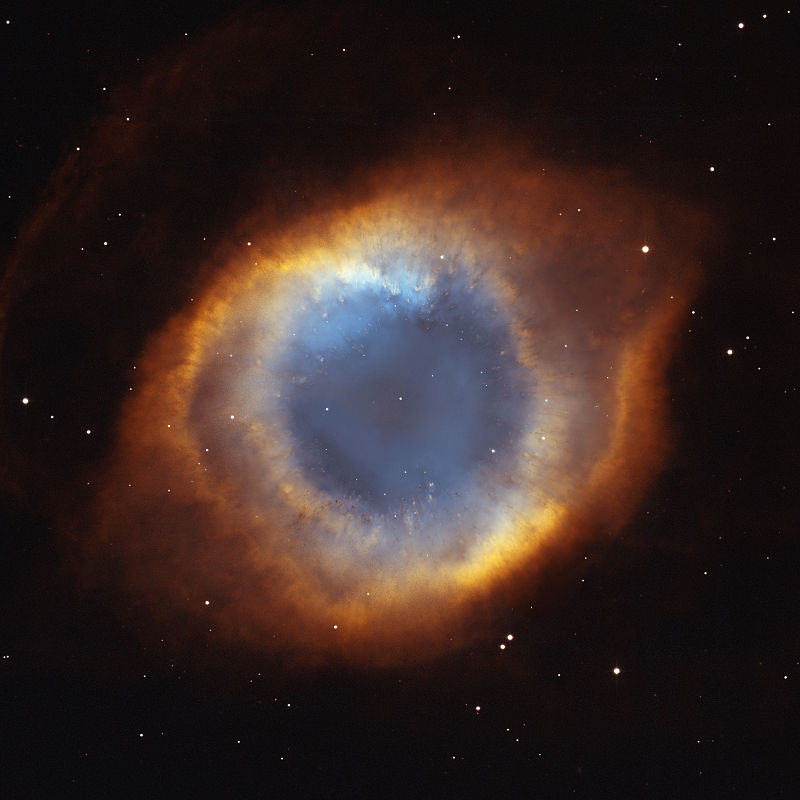
\includegraphics[scale=0.3]{nebuleuse}
    \caption{Nébuleuse planétaire de l’hélice, résultat de l'effondrement d'une étoile, en son centre siège une naines blanche  Source : \url{https://fr.wikipedia.org/wiki/Nébuleuse_planétaire}}
\end{figure}

\section{Théorie des naines blanches}
Par soucis de compréhension nous ferons l'approximation qu'une naine blanche à un rayon équivalent à celui de la Terre $5000 km$ une masse équivalente à celle du Soleil $10^{30}kg$ et donc une densité de $5.10^{6}g.cm^{-3}$, les naines blanches font parties des objet les plus dense de l'univers et ne sont dépassée que par des objet tel que les étoiles à neutron par exemple.





\end{document}
